\documentclass[bachelor, och, labwork]{shiza}
% параметр - тип обучения - одно из значений:
%    spec     - специальность
%    bachelor - бакалавриат (по умолчанию)
%    master   - магистратура
% параметр - форма обучения - одно из значений:
%    och   - очное (по умолчанию)
%    zaoch - заочное
% параметр - тип работы - одно из значений:
%    referat    - реферат
%    coursework - курсовая работа (по умолчанию)
%    diploma    - дипломная работа
%    pract      - отчет по практике
% параметр - включение шрифта
%    times    - включение шрифта Times New Roman (если установлен)
%               по умолчанию выключен
\usepackage{subfigure}
\usepackage{tikz,pgfplots}
\pgfplotsset{compat=1.5}
\usepackage{float}

%\usepackage{titlesec}
\setcounter{secnumdepth}{4}
%\titleformat{\paragraph}
%{\normalfont\normalsize}{\theparagraph}{1em}{}
%\titlespacing*{\paragraph}
%{35.5pt}{3.25ex plus 1ex minus .2ex}{1.5ex plus .2ex}

\titleformat{\paragraph}[block]
{\hspace{1.25cm}\normalfont}
{\theparagraph}{1ex}{}
\titlespacing{\paragraph}
{0cm}{2ex plus 1ex minus .2ex}{.4ex plus.2ex}

% --------------------------------------------------------------------------%


\usepackage[T2A]{fontenc}
\usepackage[utf8]{inputenc}
\usepackage{graphicx}
\graphicspath{ {./images/} }
\usepackage{tempora}

\usepackage[sort,compress]{cite}
\usepackage{amsmath}
\usepackage{amssymb}
\usepackage{amsthm}
\usepackage{fancyvrb}
\usepackage{listings}
\usepackage{listingsutf8}
\usepackage{longtable}
\usepackage{array}
\usepackage[english,russian]{babel}

\usepackage[colorlinks=false]{hyperref}
\usepackage{url}

\usepackage{underscore}
\usepackage{setspace}
\usepackage{indentfirst} 
\usepackage{mathtools}
\usepackage{amsfonts}
\usepackage{enumitem}
\usepackage{tikz}
\usepackage{minted}

\newcommand{\eqdef}{\stackrel {\rm def}{=}}
\newcommand{\specialcell}[2][c]{%
\begin{tabular}[#1]{@{}c@{}}#2\end{tabular}}

\renewcommand\theFancyVerbLine{\small\arabic{FancyVerbLine}}

\newtheorem{lem}{Лемма}

\begin{document}

% Кафедра (в родительном падеже)
\chair{теоретических основ компьютерной безопасности и криптографии}

% Тема работы
\title{Проверка чисел на простоту}

% Курс
\course{5}

% Группа
\group{531}

% Факультет (в родительном падеже) (по умолчанию "факультета КНиИТ")
\department{факультета КНиИТ}

% Специальность/направление код - наименование
%\napravlenie{09.03.04 "--- Программная инженерия}
%\napravlenie{010500 "--- Математическое обеспечение и администрирование информационных систем}
%\napravlenie{230100 "--- Информатика и вычислительная техника}
%\napravlenie{231000 "--- Программная инженерия}
\napravlenie{100501 "--- Компьютерная безопасность}

% Для студентки. Для работы студента следующая команда не нужна.
% \studenttitle{Студентки}

% Фамилия, имя, отчество в родительном падеже
\author{Улитина Ивана Владимировича}

% Заведующий кафедрой
% \chtitle{} % степень, звание
% \chname{}

%Научный руководитель (для реферата преподаватель проверяющий работу)
\satitle{профессор} %должность, степень, звание
\saname{В. А. Молчанов}

% Руководитель практики от организации (только для практики,
% для остальных типов работ не используется)
% \patitle{к.ф.-м.н.}
% \paname{С.~В.~Миронов}

% Семестр (только для практики, для остальных
% типов работ не используется)
%\term{8}

% Наименование практики (только для практики, для остальных
% типов работ не используется)
%\practtype{преддипломная}

% Продолжительность практики (количество недель) (только для практики,
% для остальных типов работ не используется)
%\duration{4}

% Даты начала и окончания практики (только для практики, для остальных
% типов работ не используется)
%\practStart{30.04.2019}
%\practFinish{27.05.2019}

% Год выполнения отчета
\date{2023}

\maketitle

% Включение нумерации рисунков, формул и таблиц по разделам
% (по умолчанию - нумерация сквозная)
% (допускается оба вида нумерации)
% \secNumbering

%-------------------------------------------------------------------------------------------

\section{Постановка задачи}

    \textbf{Цель работы} - изучение основных методов проверки простоты чисел и
    их программная реализация. 

    Порядок выполнения работы:
    \begin{enumerate}
        \item Рассмотреть тест Ферма проверки чисел на простоту и привести его
        программную реализацию;
        \item Рассмотреть тест Соловея-Штрассена проверки чисел на простоту и
        привести его программную реализацию;
        \item Рассмотреть тест Миллера-Рабина и привести его программную
        реализацию;
    \end{enumerate}

\section{Теоретические сведения}

    \subsection{Детерминированные алгоритмы проверки чисел на простоту}

        \underline{Решето Эратосфена.} Построение простых чисел, не
        превосходящих заданного числа N.

        \underline{Критерий Вильсона.} Для любого $n \in \mathbb{N}$ следующие
        условия эквивалентны:

        \begin{enumerate}
            \item $n$ "--- простое,
            \item $(n - 1)! \equiv -1 \pmod n$.
        \end{enumerate}

    \subsection{Вероятностные алгоритмы проверки чисел на простоту}

        Вероятностный алгоритм проверки числа $n$ на простоту использует
        необходимое условие простоты $P(a)$:

        \begin{enumerate}
            \item выбирается случайным образом $1 < a < n$ и проверяется
            выполнимость теста $P(a)$ "--- некоторого условия алгоритма,
            \item если тест не проходит, т.е. $P(a)$ не выполняется, то вывод
            ''число составное'',
            \item если тест проходит, т.е. $P(a)$ выполняется, то вывод ''число,
            вероятно, простое''.
        \end{enumerate}

        Если событие $A$ "--- ''число $n$ простое'' имеет вероятность $ P(A) >
        \frac{1}{2}$, то вероятность ошибки "--- получить для составного числа
        $n$ вывод ''число $n$ возможно простое'' $P(\overline{A}) < \frac{1}{2}$
        и при $t$ повторах теста вероятность ошибки $P(\overline{A}^t) <
        \frac{1}{2^t} \approx 0.$

        \subsubsection{Тест Ферма}

            \underline{Малая теорема Ферма.} Если $p$ "--- простое число, то для
            любого $a \in Z^*_p$ выполняется свойство $F_p (a) = (a^{p - 1}
            \equiv 1 \pmod p).$

            $p$ "--- простое число $\Longrightarrow F^+_p = Z^*_n,$

            где $F^+_p = \{a \in Z^*_p : F_p (a)\}$ "--- множество
            истинности предиката $F_p (a).$

            \underline{Определение.} Число $n$ называется псевдопростым по основанию
            $a \in Z^*_n$, если выполняется $F_n (a).$ Здесь $F^+_n = \{a
            \in Z^*_n | F_n (a)\}.$

            \underline{Лемма 1.} Для нечетного числа $n$ справедливы утверждения:

            \begin{enumerate}
                \item $F^+_n$ "--- подгруппа $Z^*_n$;
                \item если $F^+_n \neq Z^*_n$, то по теореме Лагранжа
                
                $$|Z^*_n| = |F^+_n| \cdot |Z^*_n / F^+_n| \geq 2 \cdot |F^+_n|,
                \text{  } |F^+_n| \leq \frac{|Z^*_n|}{2}.$$

                Вероятность успеха "--- вероятность получить ''Число $n$ составное''
                для составного числа $n$ равна $P_0 = 1 - \frac{|F^+_n|}{n - 1}.$
            \end{enumerate}

            Возможны три случая:

            \begin{enumerate}
                \item число $n$ простое и тест всегда дает ответ ''Число $n$,
                вероятно, простое'';
                \item число $n$ составное и $F^+_n \neq Z^*_n$, тогда тест дает
                ответ ''Число $n$ составное'' с вероятностью успеха

                $$P_0 = 1 - \frac{|F^+_n|}{n - 1} \geq 1 - \frac{|F^+_n|}{|Z^*_n|}
                \geq 1 - \frac{1}{2} = \frac{1}{2};$$

                \item число $n$ составное и $F^+_n = Z^*_n$, тогда тест дает ответ
                ''Число $n$ составное'' с вероятностью успеха $P_0 = 1 -
                \frac{\varphi(n)}{n - 1}.$

                Во втором случае при $k$ повторах теста вероятность успеха
                $$P_0^{(k)} = 1 - (1 - P_0)^k \geq 1 - \frac{1}{2^k} \approx 1.$$ 
            \end{enumerate}

        \subsubsection{Числа Кармайкла}

            \underline{Определение.} Нечетное составное число $n$ называется
            числом Кармайкла, если $F^+_n = Z^*_n$ (и, значит, вероятность
            успеха теста простоты на основе малой теоремы Ферма будет $P_0 = 1 -
            \frac{\varphi(n)}{n - 1}$).

            \underline{Лемма 2.} Для любого числа Кармайкла $n$ справедливы
            утверждения:

            \begin{enumerate}
                \item $n = p_1 p_2 \dots p_k$ для $k \geq 3$ простых различных
                чисел $p_1 p_2 \dots p_k$;
                \item ($\forall p$ "--- простое) $p | n \Rightarrow p - 1 | n - 1.$
            \end{enumerate}

            Количество чисел Кармайкла $k \leq n: C(n) > n^{\frac{2}{7}}.$

        \subsubsection{Тест Соловея-Штрассена}

            \underline{Критерий Эйлера.} Нечетное число $n$ является простым
            тогда и только тогда, когда для любого $a \in Z^*_n$ выполняется
            свойство

            $$E_n (a) = \left(a^{\frac{n - 1}{2}} \equiv
            \left(\frac{a}{n}\right) \pmod n \right).$$

            $n$ "--- простое число $\Longleftrightarrow F^+_n = Z^*_n$, где 

            $$E^+_n = \{a \in Z^*_n \text{ } | \text{ } E_n (a) \}.$$

            \underline{Определение.} Число $n$ называется эйлеровым
            псевдопростым по основанию $a \in Z^*_n,$ если выполнения $E_n (a).$

            \underline{Лемма 1.} Для нечетного числа $n$ справедливы утверждения:

            \begin{enumerate}
                \item $E^+_n$ "--- подгруппа $Z^*_n$;
                \item Если $n$ "--- составное число, то $|E^+_n| \leq \frac{|Z^*_n|}{2}$
            \end{enumerate}

            Вероятность успеха тест простоты Соловея-Штрассена на основе
            критерия Эйлера для составного числа $n$ равна $P_0 = 1 -
            \frac{|E^+_n|}{n - 1} \geq \frac{1}{2}.$

            Возможны два случая:

            \begin{enumerate}
                \item число $n$ простое и тест всегда дает ответ ''Число $n$,
                вероятно, простое'';
                \item число $n$ составное и тест дает ответ ''Число $n$
                составное'' с вероятностью успеха $P_0 \geq \frac{1}{2}$.

                Во втором случае при $k$ повторах теста вероятность успеха
                
                $$P_0^{(k)} = 1 - (1 - P_0)^k \geq 1 - \frac{1}{2^k} \approx
                1.$$
            \end{enumerate}


        \subsubsection{Тест Миллера-Рабина}

            \underline{Теорема (Критерий Миллера).} Пусть $n$ "--- нечетное
            число и $n - 1 = 2^s t$ для нечетного $t$. Тогда $n$ является
            простым в том и только том случае, если для любого $a \in Z^*_n$
            выполняется свойство

            $$M_n (a) = \left(a^t \equiv 1 \pmod n \vee (\exists 0 \leq k < s) (a^{2^k t}) \equiv -1 \pmod n \right).$$

            $n$ "--- просто число $\Longleftrightarrow M^+_n = Z^*_n$, где

            $$M^+_n = \{a \in Z^*_n \text{ } | \text{ } M_n (a)\}.$$

            \underline{Определение.} Число $n$, псевдопростое по основанию $a
            \in Z^*_n$, называется сильно псевдопростым по этому основанию $a
            \in Z^*_n$, если выполняется $M_n (a)$, т.е. выполняется одно из
            условий:

            \begin{enumerate}
                \item либо $a^t \equiv 1 \pmod n$;
                \item либо $a^{2^k t} \equiv -1 \pmod n$ для некоторого $0 \leq
                k < s$.
            \end{enumerate}

            Для составного числа $n$ выполняется $|M^+_n| \leq
            \frac{|Z^*_n|}{4}$ и, значит, вероятность успеха теста простоты
            Миллера-Рабина на основе критерия Миллера для составного числа $n$
            равна $P_0 = 1 - \frac{|M^+_n|}{n - 1} \geq \frac{3}{4}.$ При $k$
            повторах теста вероятность успеха 

            $$P_0^{(k)} = 1 - (1 - P_0)^k \geq 1 - \frac{1}{4^k} \approx 1.$$


        \subsubsection{Сравнение тестов простоты чисел}

            $$M_n (a) \Longrightarrow E_n (a) \Longrightarrow F_n (a) \text{ и,
            значит, } M^+_n \subset E^+_m \subset F^+_n.$$

\section{Результаты работы}

    \subsection{Описание алгоритма разложения чисел в цепную дробь и алгоритмов
    приложений цепных дробей}

        \underline{Алгоритм 1 - тест простоты на основе малой теоремы Ферма}\\
            \textit{Вход}: Нечетное число $n > 5$.\\
            \textit{Выход}: ''Число $n$, вероятно, простое'' или ''Число $n$ составное''.\\
            \underline{Шаг 1.} Выбрать случайно $a \in \{1, 2, \dots, n - 1\}$ и
            вычислить $d = $ НОД$(a, n).$ Если $d > 1,$ то ответ ''Число $n$ составное''.\\
            \underline{Шаг 2.} Если $d = 1$, то проверить условие
            $$F_n (a) = (a^{n - 1} \equiv 1 \pmod n).$$ Если оно не выполнено,
            то ответ ''Число $n$ составное''. В противном случае ответ ''Число
            $n$, вероятно, простое''.\\
            
        \underline{Псевдокод:}
            \begin{minted}[breaklines,fontsize=\small]{text}
            функция Тест_Ферма(число):
                a = случайное_число_в_диапазоне(1, число - 1)
            
                если НОД(a, число) == 1 то
                    powered_a = в_степень_по_модулю(a, число - 1, число)
                    если powered_a == 1 то
                        Вывести "Число", число, "вероятно, простое."
                    иначе
                        Вывести "Число", число, "составное."
                    конец если
                иначе
                    Вывести "Число", число, "составное."
                конец если              
            \end{minted}

            Трудоемкость алгоритма $O(\log^3(n))$.\\

        \underline{Алгоритм 2 - тест простоты Соловея-Штрассена}\\
            \textit{Вход}: Нечетное число $n > 5$.\\
            \textit{Выход}: ''Число $n$, вероятно, простое'' или ''Число $n$ составное''.\\
            \underline{Шаг 1.} Выбрать случайно $a \in \{1, 2, \dots, n - 1\}$ и
            вычислить $d = $ НОД$(a, n).$ Если $d > 1,$ то ответ ''Число $n$ составное''.\\
            \underline{Шаг 2.} Если $d = 1$, то проверить условие $E_n (a)$.
            Если оно не выполнено, то ответ ''Число $n$ составное''. В противном
            случае ответ ''Число $n$, вероятно, простое''.\\
            
        \underline{Псевдокод:}
            \begin{minted}[breaklines,fontsize=\small]{text}
            функция Тест_Соловея_Штрассена(число):
                a = случайное_число_в_диапазоне(1, число - 1)
            
                если НОД(a, число) == 1 то
                    powered_a = в_степень_по_модулю(a, (число - 1) / 2, число)
                    a_n = символ_Якоби(a, число)
                    если powered_a == a_n.взято_по_модулю(число) то
                        Вывести "Число", число, "вероятно, простое."
                    иначе
                        Вывести "Число", число, "составное."
                    конец если
                иначе
                    Вывести "Число", число, "составное."
                конец если
                         
            \end{minted}

            Трудоемкость алгоритма $O(\log^3(n))$.\\


        \underline{Алгоритм 3 - тест простоты Миллера-Рабина}\\
            \textit{Вход}: Нечетное число $n > 5$.\\
            \textit{Выход}: ''Число $n$, вероятно, простое'' или ''Число $n$ составное''.\\
            \underline{Шаг 1.} Выбрать случайно $a \in \{1, 2, \dots, n - 1\}$ и
            вычислить $d = $ НОД$(a, n).$ Если $d > 1,$ то ответ ''Число $n$ составное''.\\
            \underline{Шаг 2.} Если $d = 1$, то вычислить $r_k = a^{2^k t}$ для
            значений $k \in \{0, 1, 2, \dots, s - 1\}$. Если $r_0 \equiv 1 \pmod
            n$ или $r_k \equiv -1 \pmod n$ для некоторого $0 \leq k < s$, то
            ответ ''Число $n$, вероятно, простое''. В противном случае ответ
            ''Число $n$ составное''.\\

        \underline{Псевдокод:}
            \begin{minted}[breaklines,fontsize=\small]{text}
            функция Тест_Миллера_Рабина(число):
                a = случайное_число_в_диапазоне(1, число - 1)

                если НОД(a, число) == 1 то
                    t = число - 1
                    s = 0
                    пока t % 2 == 0 делать
                        t = t / 2
                        s = s + 1
                    конец пока
            
                    r_0 = в_степень_по_модулю(a, t, число)
                    если r_0 != 1 и r_0 != (число - 1) то
                        Вывести "Число", число, "составное."
                        вернуть
                    конец если
            
                    для k от 1 до (s - 1) делать
                        r_k = в_степень_по_модулю(a, 2^k * t, число)
                        если r_k != (число - 1) то
                            Вывести "Число", число, "составное."
                            вернуть
                        конец если
                    конец для
            
                    Вывести "Число", число, "вероятно, простое."
                иначе
                    Вывести "Число", число, "составное."
                конец если
            \end{minted}

            Трудоемкость алгоритма $O(\log^3(n))$.\\
    
    \subsection{Код программы, реализующей рассмотренные алгоритмы}

        \inputminted[breaklines,fontsize=\small,linenos]{rust}{../code/src/main.rs}

    \subsection{Результаты тестирования программ}
        \begin{figure}[H]
            \centering
            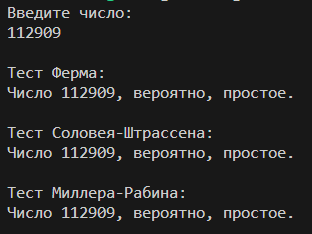
\includegraphics[width=0.8\textwidth]{pic/1.png}
            \caption{Первый тест алгоритмов проверки чисел на простоту}
        \end{figure}

        \begin{figure}[H]
            \centering
            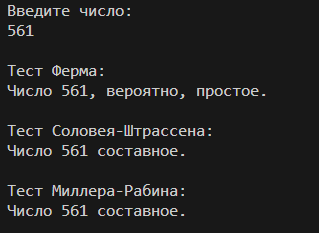
\includegraphics[width=0.8\textwidth]{pic/2.png}
            \caption{Второй тест алгоритмов проверки чисел на простоту}
        \end{figure}

        \begin{figure}[H]
            \centering
            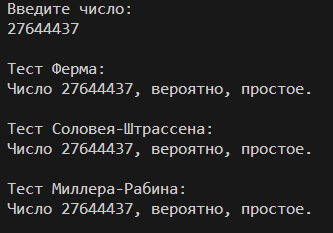
\includegraphics[width=0.8\textwidth]{pic/3.png}
            \caption{Третий тест алгоритмов проверки чисел на простоту}
        \end{figure}

\conclusion

    В данной лабораторной работе были изучены теоретические сведения о методах
    проверки простоты чисел (тест Ферма, Соловея-Штрассена, Миллера-Рабина). На
    их основе были рассмотрены соответствующие алгоритмы. Была произведена
    оценка сложности созданных алгоритмов. Они послужили фундаментом для
    программной реализации, которая впоследствии успешно прошла тестирование,
    результаты которого были прикреплены к отчету вместе с листингом программы,
    написанной на языке Rust с использованием стандартных библиотек языка.

\end{document}
